\documentclass[compress]{beamer}

\usepackage[nofonts]{ctex}
\setCJKmainfont[ItalicFont={Kaiti SC}]{Kaiti SC}%
%\setCJKmainfont[ItalicFont={AR PL KaitiM GB}]{AR PL KaitiM GB}%
%\setCJKsansfont{WenQuanYi Zen Hei}% 文泉驿的黑体

\mode<beamer>
{
    \useinnertheme{rounded}
    %\useoutertheme{miniframes}
     \useoutertheme{split}
     %\usecolortheme{orchid}
     %\usecolortheme{whale}
     %\usecolortheme{lily}
     \usecolortheme{rose}
     \usecolortheme{seahorse}

     \expandafter\def\expandafter\insertshorttitle\expandafter{%
       \insertshorttitle\hfill%
       \insertframenumber\,/\,\inserttotalframenumber}
}

\mode<handout>
{
	\usetheme{default}
	\usepackage{pgfpages}
	\pgfpagesuselayout{4 on 1}[a4paper,landscape,border shrink=5mm]
}


\usepackage{amsmath,latexsym,amssymb,amsfonts,amsbsy}
\usepackage{graphicx}
\usepackage{hyperref}
\usepackage{listings}

\setbeamercolor{dblue}{fg=white,bg=blue!30!gray} % for beamercolorbox
\newenvironment{pblock}{\begin{beamercolorbox}[rounded=true,
        shadow=true]{dblue}}{\end{beamercolorbox}}


\newcommand{\romannumber}[1]{{\textrm{\uppercase\expandafter{\romannumeral
#1}}}}

\graphicspath{{figure/}}

\lstset{
	basicstyle=\tiny, % print whole listing footnotesize
	keywordstyle=\tiny\color{black}\bfseries, 
	identifierstyle=\tiny\color{blue}, 
	commentstyle=\tiny\itshape, 
	stringstyle=\tiny\ttfamily,
	frame=single, 
	numbers=left, numberstyle=\tiny,
	stepnumber=1, numbersep=10pt,
	showtabs=false, tabsize=4,
	showstringspaces=false,
	breaklines=true, breakatwhitespace=true,
	language=[ISO]C++
}   


%%%%%%%%%%%%%%%%%%%%%%%%%%%%%%%%%%%%%%%%%%%%%%%%%%%%%%%%%%%%%%%%%
%    body                                                       %
%%%%%%%%%%%%%%%%%%%%%%%%%%%%%%%%%%%%%%%%%%%%%%%%%%%%%%%%%%%%%%%%%


\begin{document}

\AtBeginSection[]
{ 
    \begin{frame}<beamer> 
		\frametitle{内容提要} 
		\tableofcontents[currentsection,currentsubsection] 
	\end{frame} 
} 
					
\title{Unix文化与哲学}

\author[\href{http://c.pku.edu.cn/}{http://c.pku.edu.cn/}]
{曹东刚\\\href{mailto:caodg@sei.pku.edu.cn}{caodg@sei.pku.edu.cn}}

\institute[北大信科]{Linux程序设计环境 \\
\href{http://c.pku.edu.cn/}{
http://c.pku.edu.cn/}}

\date{}

\titlegraphic{\includegraphics[height=0.17\textwidth]{Overlays/logo.pdf}}

\begin{frame}
	\titlepage
\end{frame}

\section{Unix 文化}

\begin{frame}
\frametitle{工程领域的文化 }
\begin{itemize}
    \item 大多数工程领域都有自己的技术文化
        \begin{itemize}
        \item 不成文的知识, 传统, 约定, \ldots
        \item 口口相传
        \end{itemize}
    \item 软件技术领域有所不同
        \begin{itemize}
        \item 技术变化太快, 缺少稳定的技术文化
        \end{itemize}
    \item Unix是软件技术领域中的特例
        \begin{itemize}
        \item  设计哲学, 编程艺术, 技术文化
        \end{itemize}
\end{itemize}

\end{frame}

\begin{frame}
\frametitle{Unix的生命力}
\begin{itemize}
\item Unix 具有极强的生命力和适应力
    \begin{itemize}
    \item 历史最长, 支持的硬件平台最多, 应用领域最广泛, \ldots
    \item Unix的核心知识经年不变: 语言, 系统调用, 工具
    \end{itemize}
\item 为什么Unix具有如此的生命力 ?
    \begin{itemize}
    \item \alert{Unix诞生之初就具有的优良设计}
    \end{itemize}
\end{itemize}
\end{frame}

\begin{frame}
\frametitle{对Unix的异议}

\begin{itemize}
\item Unix的文件模型
\item Unix的安全机制
\item Unix面向技术用户, 而不是终端用户
\item Unix的``策略与机制分离''思想
  \begin{itemize}
	\item 可选择的工具太多, 工具的选项太多
	\item 策略并不稳定, 机制是长久的
  \end{itemize}
\end{itemize}
\end{frame}


\begin{frame}
\frametitle{Unix带给我们}
\begin{itemize}
\item 丰富的开源软件
\item 活跃的开源社区
\item 平台可移植性和开放标准
\item Internet 和 WWW 
\item 高度灵活性
\item 趣味性和可玩性
\item 宝贵的经验和教训
\end{itemize}
\end{frame}

\section{Unix 哲学}

\begin{frame}
\frametitle{基本}
\begin{itemize}
\item 源起 Ken Thompson设计一个服务接口简洁、小巧精干的操作系统
\item 非正规的科班开发方法
\item 自底向上, 注重实效, 倚重经验
\end{itemize}

\end{frame}

\begin{frame}
\frametitle{Doug McIlroy的评论}
\begin{itemize}
\item 让一个程序只做好一件事
\item 程序要能协作
\item 程序要能处理文本流
\end{itemize}

\end{frame}

\begin{frame}
\frametitle{Rob Pike从C编程角度的阐述}

\begin{itemize}
\item \textbf{1:} 程序的性能瓶颈不能靠猜测得出来

\item \textbf{2:} 只有度量之后才可开始优化

\item \textbf{3:} 花哨的算法在$n$很小时通常很慢, 而 $n$通常是很小的

\item \textbf{4:} 花哨的算法比简单的算法Bug更多, 更难维护

\item \textbf{5:} 数据结构才是编程核心

\item \textbf{6:} 结束.
\end{itemize}

\end{frame}

\begin{frame}
\frametitle{Unix 哲学概览}

\begin{tabular}{|l|p{0.3\hsize}||l|p{0.3\hsize}|}
\hline

\rule[-2mm]{0mm}{10mm}\bfseries No. & \bfseries Rule of & \bfseries No. & \bfseries Rule of \\
\hline\hline

1 & Modularity & 10 & Least Surprise \\ \hline

2 & Clarity & 11 & Silence \\ \hline

3 & Composition & 12 & Repair \\ \hline

4 & Separation & 13 & Economy \\ \hline

5 & Simplicity & 14 & Generation \\ \hline

6 & Parsimony & 15 & Optimization \\ \hline

7 & Transparency & 16 & Diversity \\ \hline

8 & Robustness & 17 &Extensibility \\ \hline

9 & Representation & & \\ \hline

\end{tabular}


\end{frame}

\begin{frame}
\frametitle{模块化原则}

\begin{itemize}
\item \emph{``计算机程序设计的本质是控制复杂性''} --- Brian Kernighan

\item 软件维护至关重要且代价高昂

\item 代码模块性的发展
    \begin{itemize}
    \item 大块机器代码
 $\Longrightarrow$ 子例程 $\Longrightarrow$ 库 
$\Longrightarrow$ 进程 $\Longrightarrow$ 分布进程
    \item 然而, \emph{``没有银弹''} --- Fred Brooks
    \end{itemize}
  \item 通过模块化降低整体复杂度
\end{itemize}
\end{frame}

\begin{frame}
  \frametitle{复杂度}
  \begin{itemize}
	\item 复杂度的来源
	  \begin{itemize}
		\item 实现复杂度
		\item 接口复杂度
		\item 代码量
	  \end{itemize}
	\item 接口复杂度和实现复杂度的折中
	\item 本质的、可选的、偶然的复杂度
  \end{itemize}
  
\end{frame}

\begin{frame}
  \frametitle{复杂度的来源与映射}
  
  \centering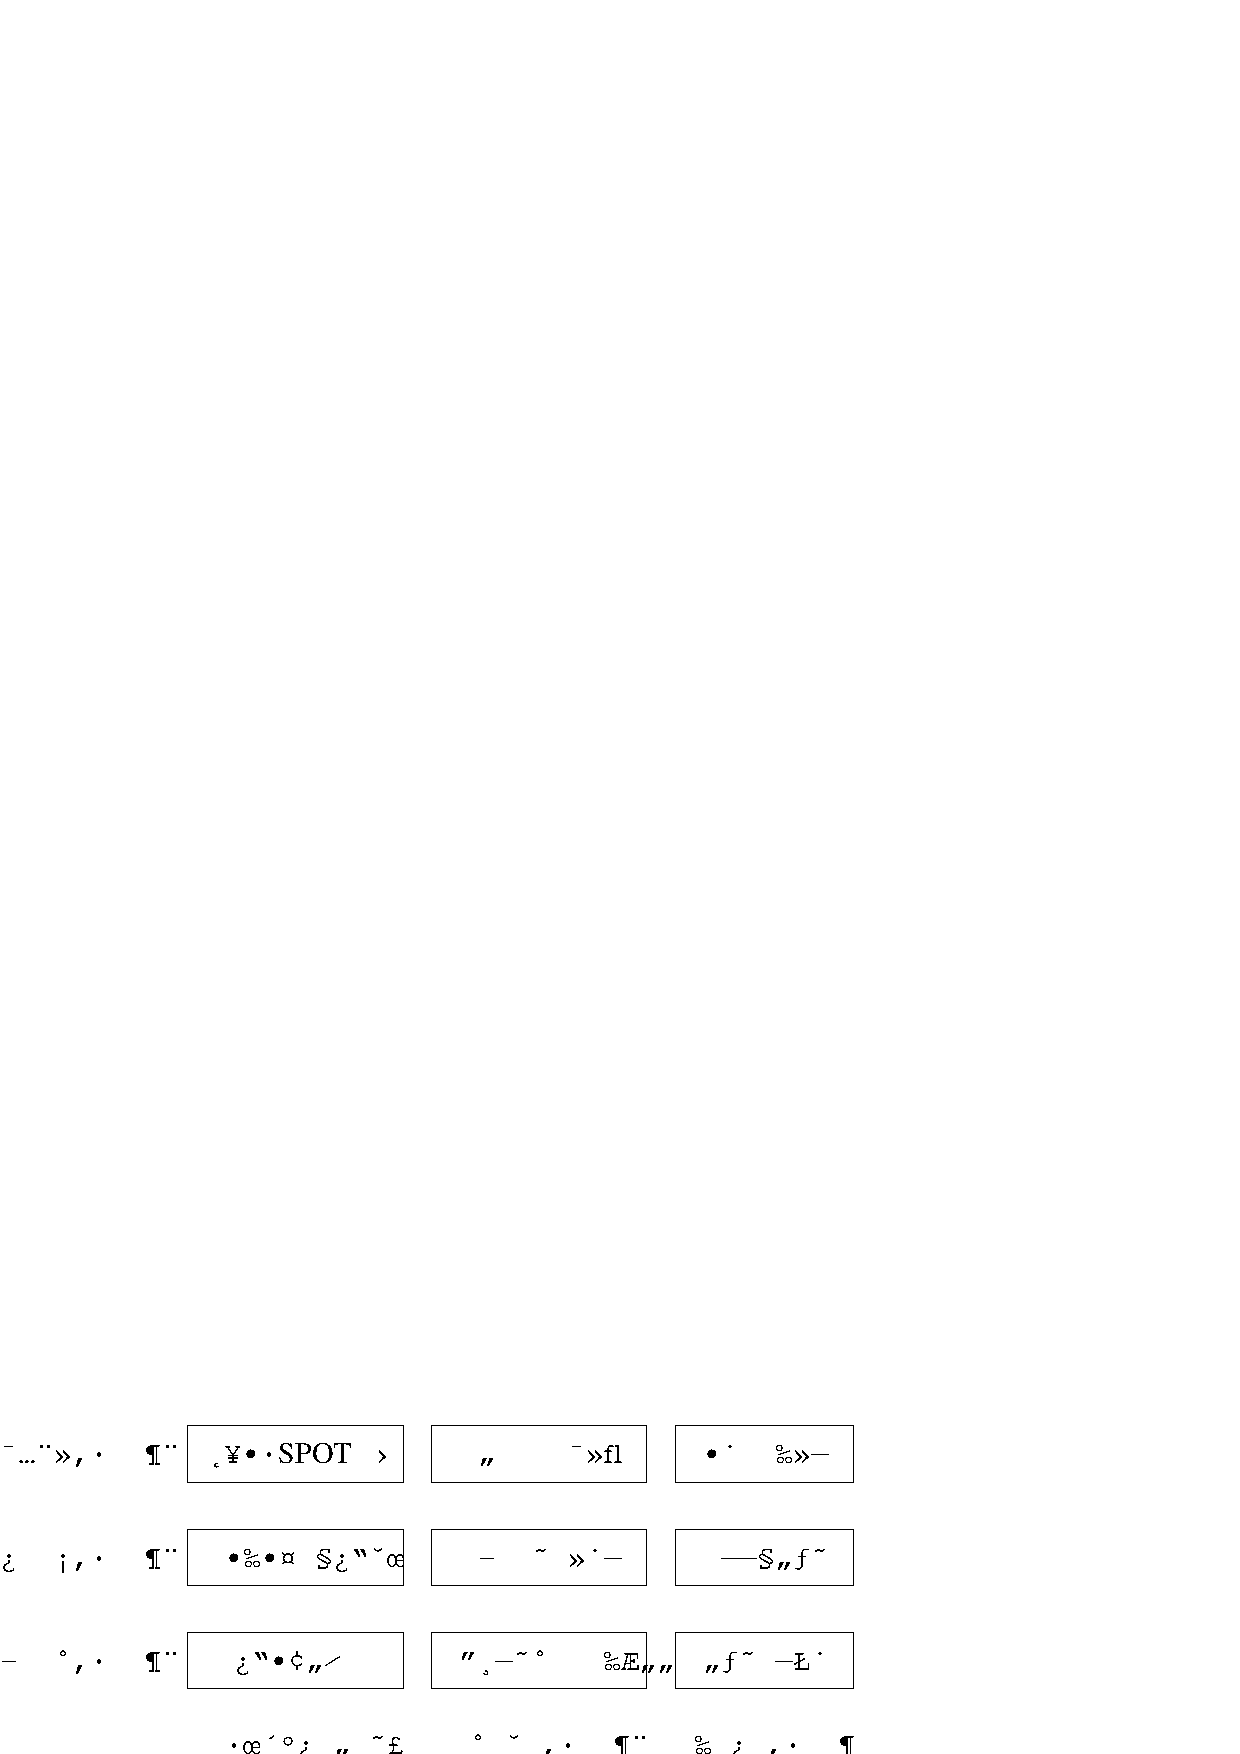
\includegraphics[width=\hsize]{complexity.pdf}
  
\end{frame}


\begin{frame}
\frametitle{清晰原则}

\begin{block}{清晰胜于机巧}
\begin{itemize}
\item 为程序员的理解、而不是机器的执行---编写代码 
\item 良好的代码注释
\item 算法尽量简单
\end{itemize}
\end{block}

\end{frame}

\begin{frame}
\frametitle{组合原则}
设计时考虑组合可组合的程序或构件

\begin{itemize}

\item 程序间的通信协议尽量为简单的文本流格式 
\vspace{-1em}
\begin{center}\includegraphics[angle=-90,width=0.8\hsize]{pipe.pdf}\\[1em]
Unix pipe-filter pattern
\end{center}

\item 程序互相独立

\item 谨慎对待GUI, 尽量避免人机过多交互

\end{itemize}
\end{frame}

\begin{frame}
\frametitle{分离原则}
\begin{block}{策略与机制分离; 接口与引擎分离}

\begin{itemize}
\item 提供引擎, 将策略留给应用\\
如: X window, GNU Hurd/Mach micro-kernel

\item 用脚本包装服务函数库\\
如: Emacs Lisp and \alert{C} library primitives

\item 前后端进程通过socket通信 \\
如: PostgreSQL server and client
\end{itemize}
\end{block}

\end{frame}

\begin{frame}
\frametitle{简洁原则与吝啬原则}

\begin{itemize}
\item 抵制编写错综复杂程序的诱惑
\item 鼓励 \emph{简洁为美}的软件设计文化
\item 除非必要, 绝不编写庞大的程序
\end{itemize}
\end{frame}

\begin{frame}
\frametitle{透明性原则}
\begin{block}{设计要可见, 以便审查和调试}

\begin{itemize}
\item 透明性: 用户可以一眼看出软件在做什么以及如何做

\item 可见性: 软件系统包含了帮助人们理解软件的功能
  \begin{itemize}
	\item 文档, 注释, 好的变量名和函数名
	\item 在设计之初就考虑加入调试功能
  \end{itemize}
  透明性和可见性使得程序便于审查和调试
\end{itemize}
\end{block}
\end{frame}

\begin{frame}
  \frametitle{如何满足透明性}
  \begin{block}{优雅的设计}
  \begin{itemize}
	\item 使用简单的输入输出格式
	\item 设计简单的接口
	\item 避免过分的抽象, 如过深的对象继承
	\item 容易找到给定函数的代码
	\item 静态调用深度最好不超过4
	\item API的函数最好正交
  \end{itemize}
 \end{block} 
\end{frame}

\begin{frame}
\frametitle{健壮性原则: 源自透明与简洁原则}

软件不仅要能在正常条件下运行良好, 在异常情况下也应能应对. 

\begin{itemize}
  \item 保持程序的内部逻辑易于理解
  \item 承受大量、极端的输入
\end{itemize}

\end{frame}

\begin{frame}
\frametitle{表示原则}
\begin{itemize}
\item 数据比算法容易驾驭
\item 如果无可选择\\
  倾向: 复杂的数据结构和简单的算法\\
  避免: 简单的数据结构和复杂的算法
\end{itemize}

\end{frame}

\begin{frame}
\frametitle{通俗原则}
\begin{block} {接口设计应避免标新立异}

\begin{itemize}
\item 切合用户已有的知识和习惯
\item 倾听和该程序相关的人员的意见
\item 尊重传统和惯例
    \begin{itemize}
    \item Unix 配置文件格式约定, 命令行开关选项, 等
    \end{itemize}
\end{itemize}
\end{block}
\end{frame}

\begin{frame}
\frametitle{缄默原则}
沉默是金: 如果程序没什么好说的, 就应保持沉默

\begin{itemize}
\item 历史: 资源宝贵
\item 技术: 有利组装
\end{itemize}
\end{frame}

\begin{frame}
\frametitle{补救原则}
{出现异常时应马上退出并给出足够的错误信息 }

\begin{itemize}
  \item 尽可能优雅地处理输入错误和自身运行错误
	\begin{itemize}
	  \item 若不能, 则尽量给出充分的诊断信息后及早退出
	\end{itemize}
  \item 接收数据宽容, 发送数据严格
\end{itemize}
\end{frame}

\begin{frame}
\frametitle{经济原则}
\begin{block}{宁花机器一分, 不花程序员一秒}
\begin{itemize}
  \item 不要重复发明轮子, 学会复用
  \item 用高级语言编程
  \item 让机器做底层的编程工作
\end{itemize}
\end{block}
\end{frame}

\begin{frame}
\frametitle{生成原则}
用程序生成程序
\begin{itemize}
\item 例如: Parser/lexer 生成器, GUI生成器,  makefile 生成器,\ldots
\end{itemize}

\end{frame}

\begin{frame}
\frametitle{优化原则}
\begin{block}{跑之前先学会走}
\begin{itemize}
\item \textit{Kernighan \& Plauger}: 90\%的功能现在能实现, 
  比100\%的功能永远实现不了强 

\item \textit{Donald Knuth}: 过早优化是万恶之源 

\item \textit{Kent Beck}: 先求运行, 再求正确, 最后求快

\item \textit{Ken Thompson}: 我最有成效的一天就是扔掉了1000行代码
\end{itemize}
\end{block}

\end{frame}

\begin{frame}
\frametitle{多样原则}

\begin{itemize}
\item 即使是最出色的软件也会受限于设计者的想象力
  \begin{itemize}
	\item 没有所谓的不二法门或永远适用的解决方案
	\item 软件不应该是封闭、僵化的
  \end{itemize}

\item Unix传统奉行: 多语言, 开放的扩展系统, 用户定制机制
\end{itemize}

\end{frame}

\begin{frame}
\frametitle{扩展原则}

\begin{itemize}
\item 为数据格式和代码留下扩展空间

\item 设计的协议或文件格式应具备自描述性

\item 应用程序的结构应组织良好, 便于扩展功能
\end{itemize}


\end{frame}

\begin{frame}
\frametitle{应用Unix哲学}

\begin{itemize}
\item 来源和目标独立的过滤器

\item 文本数据流

\item 前端和后端清晰分离

\item 用解释型语言构建原型, 之后才用C编程

\item 宽收严发

\item 小即是美

\item \ldots
\end{itemize}
\end{frame}

\section{模块化}

\begin{frame}
\frametitle{模块性}

\begin{pblock}
    保持清晰, 保持简洁
\end{pblock}

\begin{itemize}
\item Unix一直倡导模块化, 即使在其早期
    \begin{itemize}
    \item Dennis Ritchie的小把戏
    \end{itemize}

\item 评价模块的代码质量
\begin{itemize}
\item 封装性, 紧凑性, 正交性 
\end{itemize}
\end{itemize}

\begin{pblock}
    编写复杂软件的唯一方法是编写简单的各个部分, 然后通过清晰的接口将之连接起来
\end{pblock}

\end{frame}

\begin{frame}
\frametitle{封装性}
\begin{block} {良好定义的模块在封装性方面}
\begin{itemize}
  \item 不会对外暴露内部细节
  \item 不会调用其他模块的内部实现
  \item 不会胡乱共享全局数据
  \item 通过良好设计的API进行通信
\end{itemize}
\end{block}
\end{frame}

\begin{frame}
\frametitle{如何验证API是否设计良好}
\begin{itemize}
  \item 能否用自然语言描述清楚?
	\item 养成首先为接口编写注释的习惯
\end{itemize}
\end{frame}

\begin{frame}
  \frametitle{最优的模块大小}
  \centering\includegraphics[angle=-90,width=0.7\hsize]{modulesize.pdf}\\[5mm]
  \centering{缺陷数目、密度 vs. 模块大小}
\end{frame}

\begin{frame}
\frametitle{紧凑性}
\begin{block}{紧凑性:设计能否装入人脑的特性}
\begin{itemize}
\item 如何评价设计的紧凑性: 有经验的用户是否需要手册
\item 如何评价API的紧凑性: \alert{$7\pm2$} 法则
\end{itemize}
\end{block}
\end{frame}

\begin{frame}
\frametitle{程序设计工具的紧凑性}
\begin{itemize}
  \item 紧凑: make, man
  \item 半紧凑: c, python, Unix 系统调用
  \item 非紧凑: perl, java, shell
  \item 反紧凑: c++
\end{itemize}
\end{frame}

\begin{frame}
\frametitle{正交性}
\begin{block}{正交性有助于使复杂设计变得简单}
\begin{itemize}
	\item 正交系统的操作无副作用
    \item 如果不增加复杂性、引入Bug, 特定的副作用也可以接受
	\item 正交设计的例子: Unix API
    \item 非正交设计的例子: BSD sockets, X Window
	\item 避免依赖其它函数的副作用
    \end{itemize}
\end{block}
\end{frame}

\begin{frame}
\frametitle{SPOT 法则}
Single Point Of Truth, or ``Don't Repeat Yourself''

\begin{itemize}
\item 任何知识点在系统内都应该有一个唯一、明确、权威的表述.
\item 重复可能会导致矛盾、产生隐藏问题.
\item 常量、表、元数据只应声明和初始化一次.
\item 使用代码生成工具消除重复
\end{itemize}
\end{frame}

\begin{frame}
\frametitle{围绕问题明确的强力算法进行设计}

\begin{block}{良好形式化的例子}
\begin{tabular}{@{\extracolsep{3cm}}ll}
{diff} & 顺序比较 \\
{grep} & 正则表达式 \\
{lex} & 非确定有限自动机 \\
{yacc} & LR(1) 文法 \\
\end{tabular}
\end{block}

\begin{block}{启发性算法的例子}
\begin{itemize}
  \item 垃圾邮件过滤
  \item 虚拟内存管理
\end{itemize}
\end{block}

\end{frame}

\begin{frame}[containsverbatim]
	\frametitle{BSD Socket示例}
\begin{lstlisting}
#include <sys/types.h>
#include <sys/socket.h>
#include <netinet/in.h>
#include <arpa/inet.h>
#include <stdio.h>
#include <stdlib.h>
#include <string.h>
#include <unistd.h>
 
int main(void)
{
    struct sockaddr_in stSockAddr;
    int SocketFD = socket(PF_INET, SOCK_STREAM, IPPROTO_TCP);
    if(-1 == SocketFD) {
      perror("can not create socket");
      exit(EXIT_FAILURE);
    }
    memset(&stSockAddr, 0, sizeof(struct sockaddr_in));
    stSockAddr.sin_family = AF_INET;
    stSockAddr.sin_port = htons(1100);
    stSockAddr.sin_addr.s_addr = INADDR_ANY;
\end{lstlisting}
\end{frame}

\begin{frame}[containsverbatim]
	\frametitle{BSD Socket示例 (cont)}
\begin{lstlisting}[firstnumber=last]
    if(-1 == bind(SocketFD,(const struct sockaddr *)&stSockAddr, sizeof(struct sockaddr_in))) {
      perror("error bind failed");
      close(SocketFD);
      exit(EXIT_FAILURE);
    }
    if(-1 == listen(SocketFD, 10)) {
      perror("error listen failed");
      close(SocketFD);
      exit(EXIT_FAILURE);
    }
    for(;;) {
      int ConnectFD = accept(SocketFD, NULL, NULL);
      if(0 > ConnectFD) {
        perror("error accept failed");
        close(SocketFD);
        exit(EXIT_FAILURE);
      }
      shutdown(ConnectFD, SHUT_RDWR);
      close(ConnectFD);
    }
    close(SocketFD);
\end{lstlisting}
\end{frame}

\begin{frame}
\frametitle{讨论}
\begin{block}{Discussion} 
比较 Unix 和 Windows 文件操作API,谁的正交性更好? 为什么?
\end{block}
\end{frame}

\begin{frame}
\frametitle{如何帮助提高模块性}
\begin{itemize}
\item 全局变量的数目
\item 模块大小
\item 单个函数的规模
\item 有无内部API
\item API的参数
\item 模块的入口点如何分布
\end{itemize}
\end{frame}



\section{小结}

\begin{frame}
\frametitle{The Unix Philosophy in One Lesson}

\centering
\includegraphics[angle=-90,width=0.8\hsize]{kiss.pdf}

\end{frame}

\end{document}
